\section{Characterizing Extendible Partial Representations by Maximal Cliques} \label{sec:interval_orders}

In this section, we explain the characterization of extendible partial representations due to
Klav\'{\i}k et al.~\cite{kkosv}. 

\heading{Restricting Clique-points.} Suppose that there exists a representation $\calR$ extending
$\calR'$. Then $\calR$ gives some consecutive ordering $<$ of the maximal cliques from left to
right. We want to show that the pre-drawn intervals give constraints in the form of a partial
ordering $\wlt$.  Fig.~\ref{fig:simple_examples} illustrates these constraints given by a pair of
pre-drawn intervals. By generalizing it to all pre-drawn intervals, we get the partial ordering
$\wlt$.

\begin{figure}[t!]
\centering
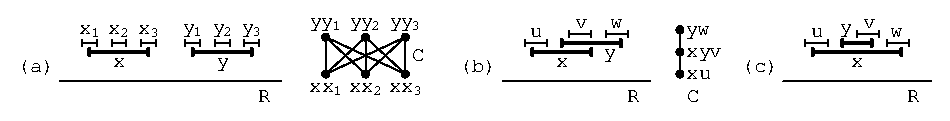
\includegraphics{interval_orders_simple_examples.eps}
\caption{Possible relative positions of pre-drawn intervals $\inter x'$ and $\inter y'$, and some
examples of the Hasse diagrams of the posed constraints. The consecutive ordering of the maximal
cliques of every extending representation has to extend $\wlt$. (a) All maximal cliques containing
$x$ have to be on the left of those containing $y$. (b) All maximal cliques containing $x$ have to
be on the left of those containing both $x$ and $y$, which are on the left of those containing only
$y$. (c) An inclusion of pre-drawn intervals poses no constraints. A maximal clique containing only
$x$ can be either on the left, or on the right of the maximal cliques containing both $x$ and $y$.}
\label{fig:simple_examples}
\end{figure}

For a maximal clique $a$, let $P(a)$ denote the set of all pre-drawn intervals that are contained in
$a$. Recall that a clique-point $\cp(a)$ is some point chosen from the intersection of all intervals
of $a$ in the representation $\calR$. Then $P(a)$ restricts the possible position of the
clique-point $\cp(a)$ to only those points $x$ of the real line which are covered in $\calR'$ by the
pre-drawn intervals of $P(a)$ and no others.  We denote the set of these admissible positions by
$\da_a$. Formally:
$$\da_a = \bigl\{ x : \text{$x \in \mathbb R$ and $x \in \inter u' \iff u \in P(a)$}\bigr\};$$
for examples see Fig.~\ref{fig:restricting_cliques}a. Equivalently, $\da_a$ is defined in~\cite{bko} as
\begin{equation} \label{eq:clique_point}
\da_a = \Bigl(\!\!\bigcap_{u \in P(a)}\!\!\! \inter u'\Bigr) \setminus
	\Bigl(\!\!\bigcup_{v \notin P(a)}\!\!\! \inter v'\Bigr).
\end{equation}

\begin{figure}[b!]
\centering
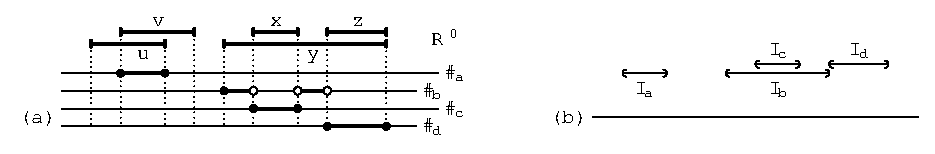
\includegraphics{interval_orders_restricting_cliques.eps}
\caption{(a) Four maximal cliques $a$, $b$, $c$, and $d$ with $P(a) = \{u,v\}$, $P(b) = \{y\}$, $P(c) =
\{x,y\}$, and $P(d) = \{y,z\}$. The possible positions $\da_a$, $\da_b$, $\da_c$, and $\da_d$ of
their clique-points are illustrated. (b) The corresponding open intervals $I_a$, $I_b$, $I_c$, and
$I_d$.}
\label{fig:restricting_cliques}
\end{figure}

We are interested in the extremal points of $\da_a$. By $\clql(a)$ (resp.~$\clqr(a)$),
we denote the infimum (resp.~the supremum) of $\da_a$.  We use an open interval $I_a =
(\clql(a),\clqr(a))$ to represent $\da_a$. We note that this does not imply that $\da_a$ contains
all points between $\clql(a)$ and $\clqr(a)$; see $\da_b$ in Fig.~\ref{fig:restricting_cliques}.
Notice that when $P(a) = \emptyset$, then $I_a = \mathbb R$.

\heading{The Interval Order $\wlt$.} For two distinct maximal cliques $a$ and $b$, we write $a \wlt
b$ if $\clqr(a) \le \clql(b)$, or in other words, if $I_a$ is on the left of $I_b$. We put $a \wlt
a$ when $\da_a = \emptyset$. The definition of $\wlt$ is quite natural, since $a \wlt b$ implies
that every extending representation $\calR$ has to place $\cp(a)$ to the left of $\cp(b)$. For
instance, in Fig.~\ref{fig:restricting_cliques}, we get that $a \wlt b \wlt d$ and $a \wlt c \wlt
d$, but $b$ and $c$ are incomparable.

We note that the ordering $\wlt$ is a so-called \emph{interval order} represented by open intervals
$I_a$. The reason is that $a \wlt b$ if and only if $I_a$ and $I_b$ are disjoint and $I_a$ is on the
left of $I_b$. Interval orders are studied in the context of time constraints and have many
applications; for instance, see~\cite{fishburn}.

\begin{lemma}[Klav\'{\i}k et al.~\cite{kkosv}] \label{lem:repext_char}
A partial representation $\calR'$ is extendible if and only if there exists a consecutive ordering of
the maximal cliques that extends $\wlt$.
\end{lemma}

It is obvious that the constraints posed by $\wlt$ are necessary. The other implication is proved
in~\cite{kkosv} as follows. Suppose that $<$ is a consecutive ordering extending $\wlt$. We place
the clique-points greedily from left to right according $<$. We place each clique-point on the right
of the previously placed ones, as far to the left as possible.
It is shown that if this greedy procedure fails, then either $<$ does not extend $\wlt$, or it is
not a consecutive ordering.

\heading{Overlaps.}
In this paper, we show one additional crucial property of $\wlt$. We say that a pair of intervals
$I_a$ and $I_b$ \emph{single overlaps} if $I_a \ne I_b$ and either $\clql(a) \le \clql(b) < \clqr(a)
\le \clqr(b)$, or $\clql(b) \le \clql(a) < \clqr(b)
\le \clqr(a)$.

\begin{lemma} \label{lem:single_overlap}
No pair of intervals $I_a$ and $I_b$ single overlaps.
\end{lemma}

\begin{proof}
Assume without loss of generality that $\clql(a) \le \clql(b)$. If $\clqr(a) \le \clql(b)$, then
$I_a$ and $I_b$ are disjoint and do not single overlap. Suppose now that $\clql(a) \le \clql(b) <
\clqr(a)$. Since all intervals of $P(a)$ cover $[\clql(a),\clqr(a)]$, we get $P(a) \subseteq P(b)$.

The position of $\clqr(a)$ can be defined as a result of two distinct situations:
\begin{packed_itemize}
\item If some pre-drawn interval of $P(a)$ ends in $\clqr(a)$, then $\clqr(b) \le \clqr(a)$, since
the same pre-drawn interval is contained in $P(b)$. 
\item Otherwise, there exists a sequence of pre-drawn intervals not contained in $P(a)$ that covers
the whole portion between $\clqr(a)$ and the leftmost right endpoint of the intervals of $P(a)$.
The left endpoints of these intervals are on or to the right of $\clqr(a)$. Since the left endpoints
of the intervals in $P(b)$ are to the left of $\clqr(a)$, the pre-drawn intervals of the sequence
are not contained in $P(b)$. Thus, $\clqr(b) \le \clqr(a)$.
\end{packed_itemize}
In both cases, $\clql(a) \le \clql(b) \le \clqr(b) \le \clqr(a)$, so $I_b$ is contained in $I_a$.\qed
\end{proof}

If no single overlaps are allowed, every pair of intervals is either disjoint, or one interval is
contained in the other (possibly the intervals are equal). This type of interval orderings is very
simple and has not been much studied. We note that graphs having interval representations with no single
overlaps are called \emph{trivially perfect}. By examining the above proof, we get the following
useful result:

\begin{lemma} \label{lem:open_intervals}
If $I_a \subseteq I_b$, then $P(a) \supseteq P(b)$. Further, strict containments correspond
to strict inclusions.\qed
\end{lemma}

If $I_a$ and $I_b$ are disjoint, then we only know that at least one of the sets $P(a) \setminus
P(b)$ and $P(b) \setminus P(a)$ is non-empty. They both might be non-empty, or the sets $P(a)$ and
$P(b)$ might be in inclusion. See Fig.~\ref{fig:restricting_cliques} for examples.

\heading{Sliding Lemma.} We introduce some notation. We denote by $P^{\endlft}(a)$ and
$P^{\startrt}(a)$ respectively the subsets of $P(a)$ containing the pre-drawn intervals with
left-most right endpoints, and with right-most left endpoints. If $u \in P^{\endlft}(a)$ and $v \in
P^{\startrt}(a)$, then $\inter u' \cap \inter v' = \bigcap_{w \in P(a)} \inter w'$, thus $I_a$ is a
subinterval of $\inter u' \cap \inter v'$.

Single overlaps of pre-drawn intervals pose more constraints than containment (see
Fig.~\ref{fig:simple_examples}b and c). Therefore, single overlaps are more powerful in building
obstructions. The following lemma states that, under some assumptions, we can turn a containment of
pre-drawn intervals into a single overlap of other pre-drawn intervals; see
Fig.~\ref{fig:sliding_lemma}.

\begin{figure}[b!]
\centering
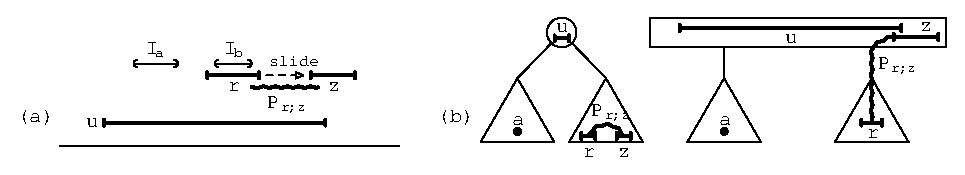
\includegraphics{interval_orders_sliding_lemma.eps}
\caption{(a) With the assumption satisfied, we can slide $r$ to $z$ which covers $r(u)$.
(b) The relative positions in the MPQ-trees of $z$ and $r$ with respect to $a$ are the same.}
\label{fig:sliding_lemma}
\end{figure}

\begin{lemma}[Sliding] \label{lem:sliding}
Let $I_a$ be on the left of $I_b$, $P(a) \subsetneq P(b)$ and $r \in P(b) \setminus P(a)$.
\begin{packed_enum}
\item[(i)]
There exists a pre-drawn interval $\inter z'$ on the right of $I_a$ covering $r(u)$, for $u \in
P^{\endlft}(a)$. Further, there exists an induced path $P_{r,z}$ from $r$ to $z$ whose vertices
are all pre-drawn and not contained in $P(a)$.
\item[(ii)]
Consider the smallest subtree having $a$ and the sections containing $r$. If the root of this subtree is
a P-node, then $z$ and $r$ are contained in the same subtree. If the root is a Q-node, then $z$ and $r$
appear on the same side of $a$.
\end{packed_enum}
\end{lemma}

\begin{proof}
(i) By the assumptions and the definition of $I_a$, we get that $(\clqr(a),r(u)]$ is not empty and
all points in $(\clqr(a),r(u)]$ are covered by pre-drawn intervals not in $P(a)$. Among these
intervals, we choose $z$ covering $r(u)$. Since $r$ is also one of these intervals, we can construct
an induced path from $r$ to $z$, consisting of pre-drawn intervals not in $P(a)$.

(ii) It follows from the existence of $P_{r,z}$ not contained in $a$.\qed
\end{proof}

We note that possibly $r = z$. The above lemma is repeatedly used for constructing minimal
obstructions. The general idea is the fact that $\inter r'$ properly contained inside $\inter u'$
restricts the partial representation less than $\inter z'$ covering $r(u)$. The lemma
says that we can assume that such $z$ exists and use it instead of $r$.

\heading{Flip Operation.} We say that we \emph{flip} the partial representation \emph{vertically}
when we map every $x \in \mathbb R$ to $-x$. This reverses the ordering $\wlt$.  Clearly, there
exists an obstruction in the original partial representation if and only if the flipped obstruction
is present in the flipped partial representation. The purpose of this operation is to decrease the
number of cases in the proofs.
